\subsection{Polarizzazione}
    \subsubsection{Legge di Malus}
        Posti emettitore e ricevitore lungo la stessa retta e inclinando attorno a tale asse l'emettitore di un angolo $\gamma$, intenità letta dal ricevitore varia, secondo la legge di Malus, come:
            $$ I = I_0 \cos^2\gamma $$
        Di seguito i dati sperimentali raccolti.
    \begin{table}[H]
    \begin{center}
    \begin{tabular}{|c|c|c|}
\hline
        $ \gamma $	&	Intensità	&	Errore I	\\
        rad	&	mA	&	mA	\\
        $ \pm 0.02 $	&	-	&	-	\\ 
        \hline
        0.00	&	7.8	    &	0.2	    \\
        0.26	&	7.2	    &	0.2	    \\
        0.52	&	8.0	    &	0.2	    \\
        0.79	&	3.4	    &	0.2	    \\
        0.87	&	2.0	    &	0.2	    \\
        0.96	&	1.20	&	0.06	\\
        1.05	&	0.51	&	0.06	\\ 
        \hline
    \end{tabular}
    \end{center}
  % \caption{}
  %  \label{O4_P2_malus}
\end{table}
%
%
%%%%%%%%%%%%%%%%%%%%%%%%%%%%%%%%%%%%%%%%%%%%%%%%%%%%%%%%%%%%
%%%%%%%%%%%%%%%%%%%%%%%%%%%%%% FIT %%%%%%%%%%%%%%%%%%%%%%%%%
%%%%%%%%%%%%%%%%%%%%%%%%%%%%%%%%%%%%%%%%%%%%%%%%%%%%%%%%%%%%
%
%
    \begin{figure}[H]
        \centering
        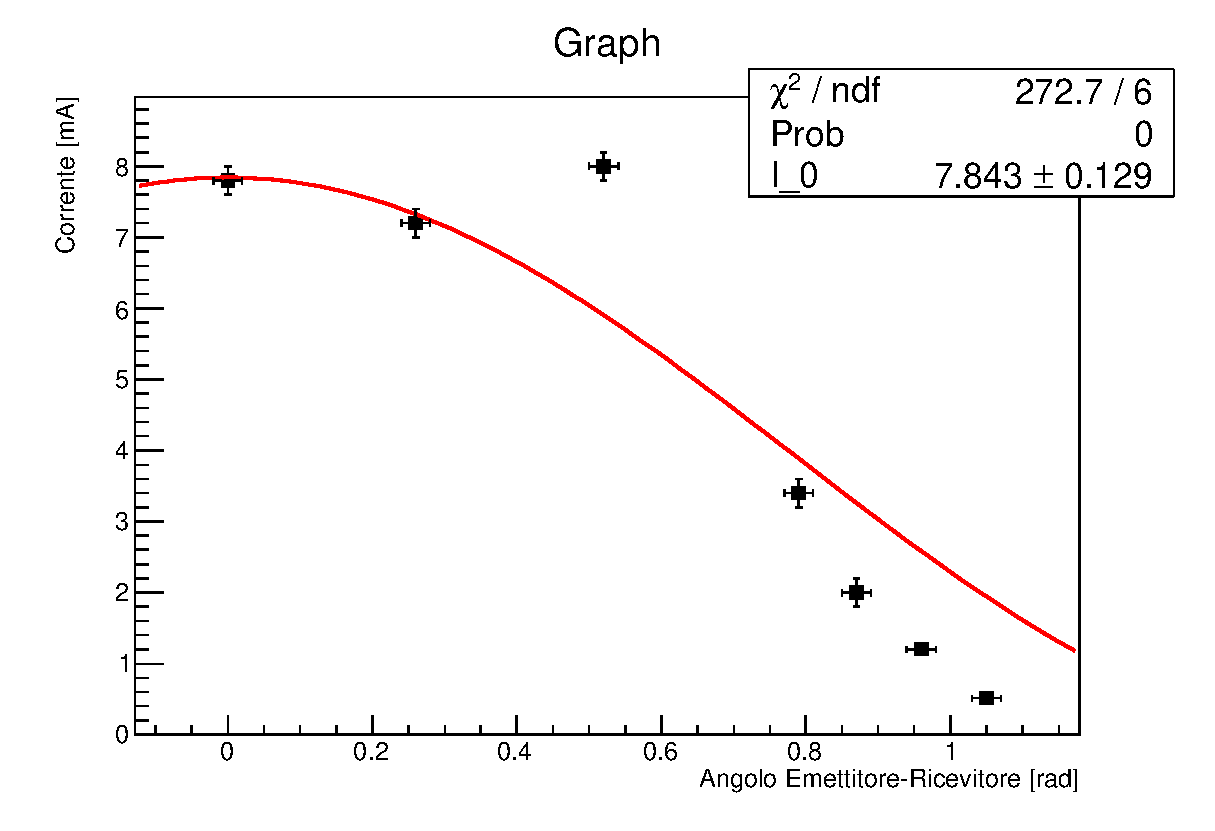
\includegraphics[scale=0.8]{Grafici/O4_P2_malus.eps}
        \caption{Fit: $ I = I_0 \cos^2\gamma $ }
        \label{fig:C3_P2_RL}
    \end{figure} 
    %\subsubsection{Filtro polarizzatore}
    %non ci è uscito
    
    \subsubsection{Angolo di Brewster}
        Non è stato possibile prendere angoli superiori a 65° per limitazioni dovute alla strumentazione. Si osserva che l'intensità della corrente tende a zero all'aumentare dell'angolo, ma non si è in grado di determinare l'angolo esatto.\\
        Supponiamo che oltre all'effetto polarizzante della riflessione sul polietilene, si verifichi anche un effetto di interferenza tra l'onda riflessa dalla superficie e l'onda che giunge diretamente da dall'emettitore, \textcolor{red}{sopratutto ad angoli grandi?}
        \begin{figure}[H]
            \centering
            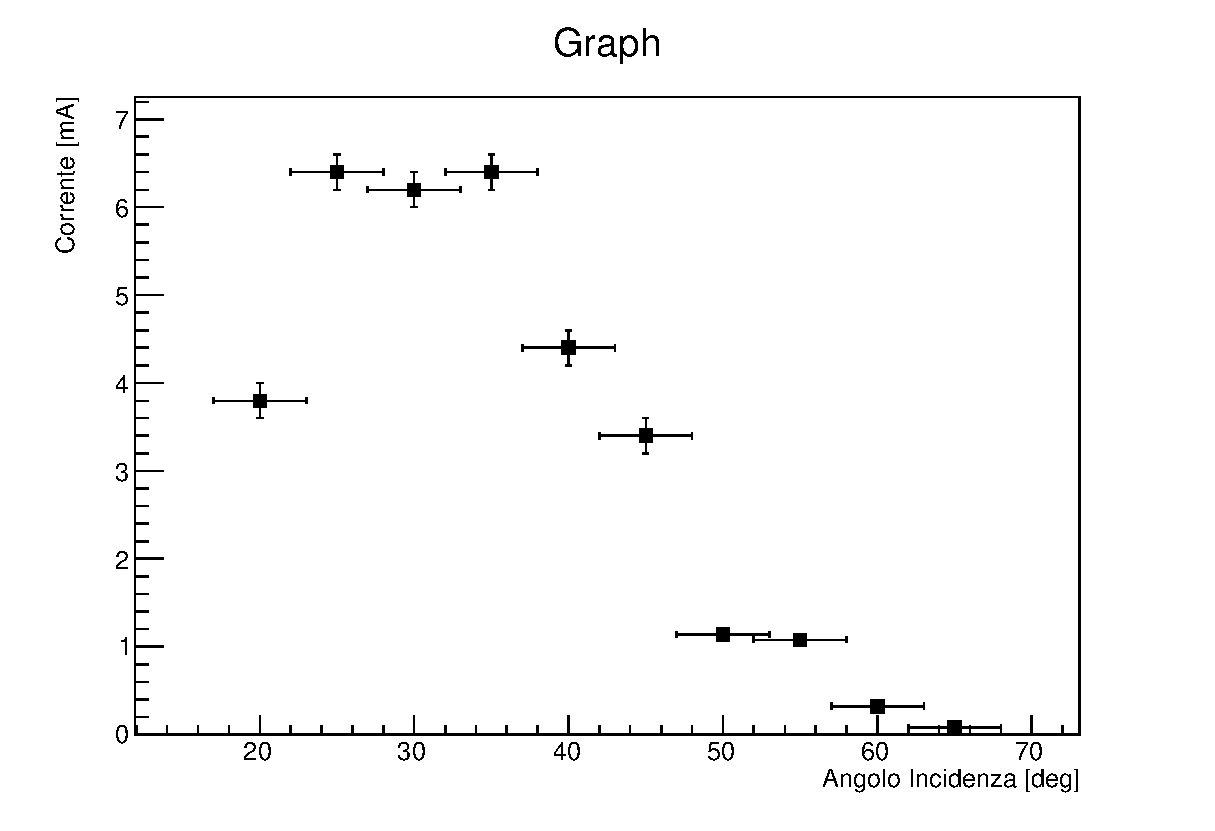
\includegraphics[scale=0.8]{Grafici/O4_P2_brewster.eps}
            \caption{Determinazione dell'angolo di Brewster}
            \label{fig:O4_P2_brewster}
        \end{figure}
